\documentclass[tikz,border=5pt]{standalone}

\usepackage{tikz}
\usepackage{sfmath}
\usetikzlibrary{arrows.meta, calc}

\begin{document}

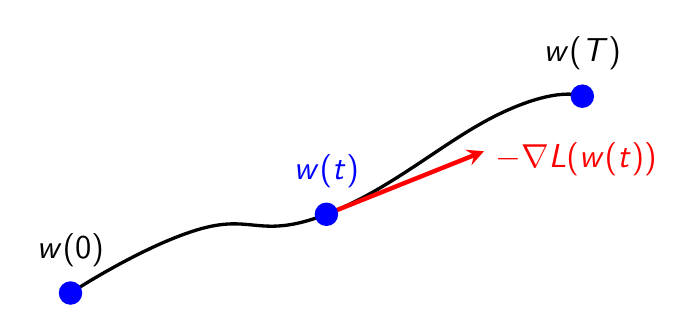
\begin{tikzpicture}[>=stealth, thick,
    point/.style={circle, fill=blue, inner sep=3pt},
    vector/.style={->, red, ultra thick},
    label_text/.style={font=\sffamily\large}
]

% Define coordinates for the trajectory
\coordinate (w0) at (0, 1.5);
\coordinate (wt) at (3.25, 2.5);
\coordinate (wT) at (6.5, 4);

% Draw the curved trajectory
\draw[black, very thick] plot [smooth, tension=0.8] coordinates {(w0) (1.6, 2.3) (wt) (5.5, 3.8) (wT)};

% Draw the points
\node[point] at (w0) {};
\node[point] at (wT) {};

% Draw and label the negative gradient vector at w(t) (drawn first so it's behind the blue dot)
% The negative gradient points in the direction of the trajectory (towards w(T))
\draw[vector] (wt) -- ($(wt) + (2, 0.8)$) node[right, red, label_text, yshift=-0.1cm] {$-\nabla L(w(t))$};

% Draw w(t) point last so it appears on top of the arrow
\node[point] at (wt) {};

% Label the points (moved up)
\node[above, label_text, yshift=0.2cm] at (w0) {$w(0)$};
\node[above, label_text, blue, yshift=0.2cm] at (wt) {$w(t)$};
\node[above, label_text, yshift=0.2cm] at (wT) {$w(T)$};

\end{tikzpicture}

\end{document}
